\section{Component Architecture}
\label{sec:components}
On the basis of section \ref{sec:systemdefinition} and our evaluation of criteria in section \ref{sec:criteria} we found that our main priority is flexibility. 
In order to obtain high flexibility we will use ASP.NET MVC 2 framework described in section \ref{sec:mvc}, to make components easily swappable.
The the application will access the database by using the ADO.NET data provider described in section \ref{sub:adonet}. This gives us a component design as seen on figure \ref{fig:system_component_mvc}.
The figure illustrates the components dependency among each other. 

\begin{figure}[h]
	\centering
		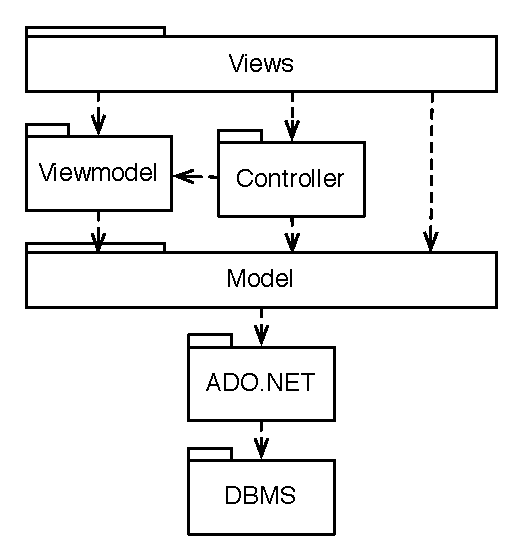
\includegraphics[scale=0.7]{input/architectural_design/system_component_mvc.pdf}
	\morscaption{The application component. The arrows represent dependency}
	\label{fig:system_component_mvc}
\end{figure}


%\begin{comment}
\paragraph{Model}
The responsibility of the model is to represent the objects and their data which is stored in- and fetched from the database. This component is further described in \ref{sub:modelComponent}.


\paragraph{Tools}
The tool component consist of various help functionality. For example the problem distributer and the search functionality is placed in this component. The tools is used by the controller and it relies on the model. 

\paragraph{View Model}
\viewmodel{}s are dependent on the model since it is a container of elements from the model.

\paragraph{View} 
Views dependent on the model, controller and \viewmodel{}. It is dependent on the controller because the views responsibility is to make buttons and links which have to match the correct controller. It is dependent on the model and \viewmodel{} because this is the data it needs to present. 
The dependency on the model could be removed and then all view data has to be parsed though a \viewmodel{}, but we allow this because it is not always necessary to put the model into a \viewmodel{}. 

\paragraph{Controller}
The controllers all have independent responsibilities, but the general responsibility of the controller components is to process the data in the model and return this to a specific view, possibly through a \viewmodel{}. The controller depends on view, model, \viewmodel{} and tool. Changing any of these components will most likely result in a change of the controller. 

\paragraph{ADO.NET}
This component is not build by us, this is an already made component which is used as a database data provider. 

%\end{comment}


\begin{comment}
%%%%%%%% Alt herunder er gammelt

created a closed-strict layers component architecture, we did this to avoid complex dependencies between components and therefore making it easy to change an interface, a function component, or \fixme{eller hvad?}. 




%system_component_mvc.pdf

The architecture has three layers: User- and Application-interfaces, Functions, Model as shown on figure \ref{fig:SystemComponent}. The figures components will be explained in section \ref{sub:SystemComponent}.

\begin{figure}
	\centering
		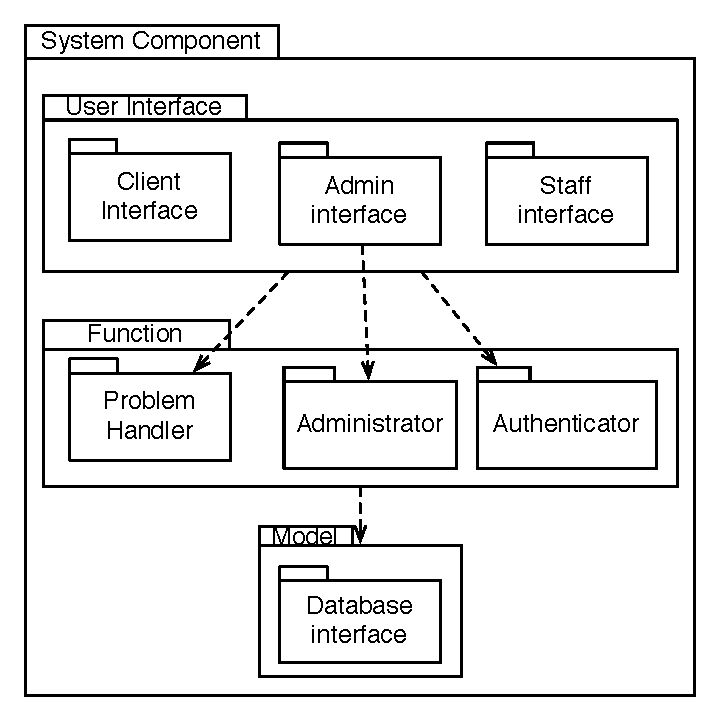
\includegraphics[scale=0.5]{input/architectural_design/system_component_denvibruger.pdf}
	\morscaption{Our application component}
	\label{fig:SystemComponent}
\end{figure}


\subsection{Application Component}
\label{sub:SystemComponent}
The application's three actors are displayed as interfaces. The \aclient s and \astaff s functions are located in the Problem Handler component, while the \admin s additional functions are located in the Administrator component. The \aclient[] only have limited access to the Problem Handler component while the \astaff[] and \admin[] have full access to the Problem Handler's functions, in addition the \admin[] uses the administrator component. To determine if a user is a \aclient[], \astaff[] or \admin[] the component Authenticator is used. The Authenticator asks the Database Interface what the permission the user have. Based on what permissions the user have access are given to the different interfaces. The Problem Handler and the Administrator components sends info to the Database Interface who translate the info and sends it to the database. All the components are described below:

\paragraph{\cinterface}
The client interface get inputs from the client, through this interface the client submits problems, post comments and search for existing problems.
The functions associated with this interface are located in the Problem Handler component.  

\paragraph{\sinterface}
Through this interface the staff members can access all the client functions, submit solutions, post comments to \open[] problems, view \worklist[] and administrate problems.
This Interface uses the Problem Handler component. 

\paragraph{\ainterface}  
The interface has access to all the \aclient[] functions, the \astaff[] functions, tags/category management, department management and administration of the client/staff. This is due to the fact that if a person is an \admin[], then he/she also is a \astaff[] and a \aclient[]. The Admin Interface uses the Problems Handler and the Administrator component. 

\paragraph{Problem Handler}
The problem handler component controls the handling of new problems, the handling of solutions, the searching function, recording and sending statistics, manages comments and sending notifications by using the notifier component.
This component is also responsible for sending out signals to relevant actors. e.g. if a user posts a comment the relevant staff member(s) receives a notification.  

\paragraph{Administrator}
Through the admin interface the admin component can be accessed. The functions affiliated with this component are control of departments, management of tags/categories and adding/removing of staffs and clients.   

\paragraph{Authenticator}
To determine which rights a person have, they have to authenticate them selves as either client or staff/admin, this occurs through an authenticator component which communicates with the database interface. 
\paragraph{Database Interface}
The database interface receives all database requests and translate them to the correct database language.

%\subsection{Alternative System component}
%\label{sub:altSystemComponent}
 
%If \hdesk[] is used by a company who already have an Active Directory, then the login system should be integrated with %the AD. We designed a component who is able to communicate with an external database\fixme{Blev vi ikke enige om at vi %ikke ville bruge external database}. As seen on figure \ref{fig:AltSystemComponent} a Login system interface component %is added. We are not going to implement this component.
%\fixme{kim: Jeg syntes det skal slettes, billedet og tekst}

%\paragraph{Login System Interface}
%The Login system interface communicates with the external database
%\begin{figure}
%	\centering
%	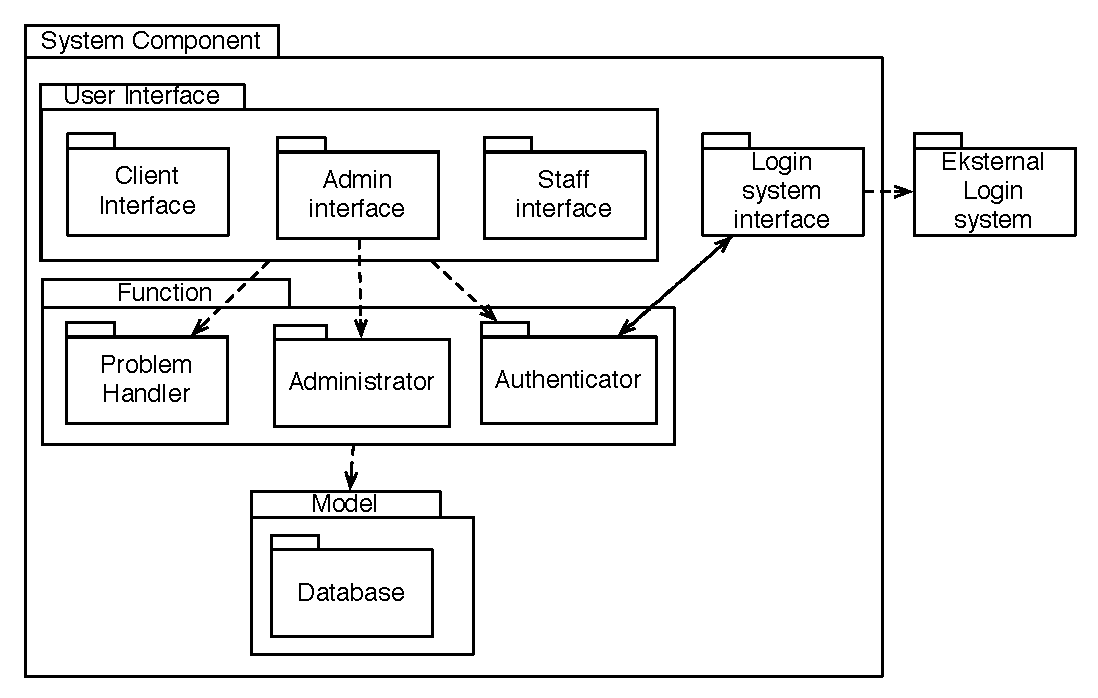
\includegraphics[scale=0.5]{input/architectural_design/system_component_denalternative.pdf}
%	\morscaption{}
%	\label{fig:AltSystemComponent}
%\end{figure}

\end{comment}


\subsection{Client-Server}
Because we are designing a help desk, we are dealing with users who are not present in a specific location. Therefore we also designed the application using a client-server architecture.
On the client side there is a user interface and on the server side the functionality and model are located as seen on figure \ref{fig:client-server}. By using Local Presentation~\cite{roedeaalborg}[p.~200] we enable clients to access the application from anywhere, and still keep the functionality and model on the server and thus keeping the application flexible.         

\vspace{-1mm}
\begin{figure}[h]%
\centering
	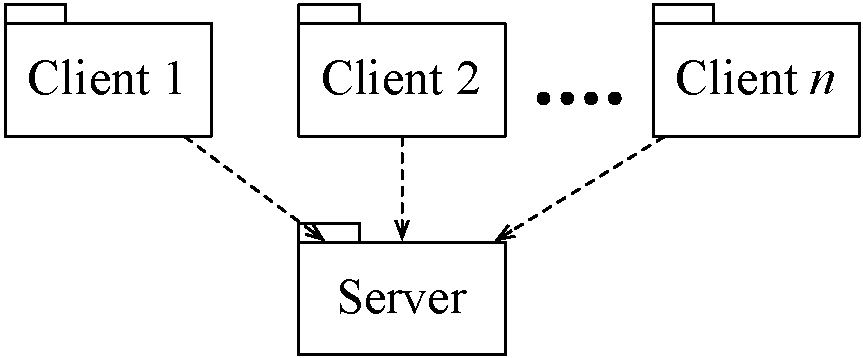
\includegraphics[scale=0.45]{input/architectural_design/client-server-architecture-pattern.pdf}%
	\morscaption{The client server design pattern}
	\label{fig:client-server}%
\end{figure}
\vspace{-5mm}